%%%%%%%%%%%%%%%%%%%%%%%%%%%%%%%%%%%%%%%%%%%%%%%%%%%%%%%%%%%%%%%%%%%%%%%%%%%%%%%%
%% BAKALÁRSKA PRÁCA                                                           %%
%%                                                                            %%
%% Názov (sk): Algoritmy detekcie a korekcie lokálnych                        %%
%%             znehodnotení digitálneho audio signálu                         %%
%% Názov (en): Algorithms for Detection and Correction of Local               %%
%%             Degradations in Digital Audio Signals                          %%
%%                                                                            %%
%% Autor: Jakub Kúdela                                                        %%
%% Vedúci: Mgr. Daniel Toropila                                               %%
%%                                                                            %%
%% Akademický rok: 2011/2012                                                  %%
%%%%%%%%%%%%%%%%%%%%%%%%%%%%%%%%%%%%%%%%%%%%%%%%%%%%%%%%%%%%%%%%%%%%%%%%%%%%%%%%

\chapwithtoc{Úvod}
Už od nepamäti zohráva zvuk zásadnú rolu v našich životoch. Nemalá časť ľudskej kultúry stavia na jeho existencii. Vypovedá o tom, čo sa deje vôkol nás a umožnuje nám medzi sebou komunikovať. Práve vďaka významnosti zvuku si ľudia našli spôsoby ako ho zaznamenať a s nimi prišli aj kvalitatívne nároky na zvukový záznam a probémy s ním späté.

\secwithtoc{História zvukového záznamu}
História zvukových záznamov siaha do polovice devätnásteho storočia. Prvé zariadenie, ktoré bolo schopné zaznamenať zvukovú stopu na papier, vynašiel francúzky  tlačiar Édouard-Léon Scott a nieslo názov fonautograf. Ďalší význámný pokrok v danej problematike priniesol americký vynálezca Thomas Alva Edison skonštruovaním aparátu s názvom fonograf. Pomocou fonografu bolo možné zvuk nielen zaznamenať na staniolom potiahnutý valec, ale ho aj reprodukovať. S podobným vynálezom, zvaným gramofón, prišiel o niekoľko rokov neskôr nemecký herec Emile Berliner. Vynájdenie gramofónu viedlo k niekoľkým zmenám materiálov využívaných na výrobu diskových nosičov a ku motorizácii prehrávacích aparátov. Všetky doposiaľ uvedené mechanizmy fungovali na princípe pohybu hrotu v záznamovej dráhe, ktorý po nabehnutí na poškodený úsek dráhy spôsoboval charakteristické praskanie. Pre mnohých poslucháčov bolo pri počúvaní zvukových záznamov praskanie nežiaduce. Iným kvalitatívnym nedostatkom všetkých doposiaľ spomenutých mechanizmov bolo relatívne úzke záznamové frekvenčné pásmo.

Zásadným krokom pre vylepšenie kvality nahrávok bola elektrifikácia nahrávacieho procesu objavená spoločnosťou Western Electric, ktorá dala podnet pre vznik magnetofónu. Mechanizmus záznamu zvuku na magnetofónovú pásku vyrobenú zo zmagnetovatelného materiálu značne vylepšil kvalitu záznamu. Zredukoval množstvo rušivých elementov v nahraných stopách a rozšíril záznamové frekvenčné pásmo z dovtedajšieho 164–2000 Hz na 20-5000 Hz. Čo sa týka poškodení na magnetofónovej páske, jej charakter umožňoval realizovať aj prvé analógové editácie. Zaznamenané nahrávky bolo možné opraviť metódou vyrezania poruchovej časti pásky a spojením jej zvyšných častí. V šesťdesiatych rokoch dvadsiateho storočia boli uvedené technológie pre analógovú úpravu zvuku ako napríklad obmedzovač hlasitosti\footnote{Preložené z anglického limiter.}, dynamický kompresor, audio filtre a ekvalizéry. Jedným zo spôsobov korekcie audio signálu, ktoré nové technológie umožňovali, bola redukcia šumu nahrávok potlačením jemu odpovedajúcich frekvencií.

Prevratným momentom v oblasti zvukového záznamu bolo uvedenie digitálneho zvuku, nosiča kompaktného disku CD a digitálnej audio pásky DAT. Digitalizácia zvuku priniesla komplexné editačné možnosti v podobe digitálneho signálového spracovania. Digitálny audio formát dnes celkom bežne poskytuje stereo záznam s 16-bitovým rozlíšením a frekvenčným pásmom do 20 kHz pri vzorkovacej frekvencií 44,1 kHz. V súčasnosti sú k dispozícií aj kvalitnejšie digitálne formáty pre profesionálne využitie.

S príchodom vysokokvalitných digitálnych audio médií sa dramaticky zvýšili všeobecné nároky na kvalitu zvukového záznamu. Záujem o historicky staršie nahrávky viedol k rastu záujmu o ich reštaurovanie. Reč je o historických nahrávkach dochovaných na starších nosičoch, ktorých kvalita odpovedá metóde, ktorou boli zaznamenané. S príchodom digitalizácie zvuku prišla aj možnost digitálneho spracovania audio signálu, ktorá dala priestor pre vznik sofistikovanejších digitálnych prístupov ku oprave zvukových nahrávok.

\secwithtoc{Znehodnotenie audio signálu}
Každé znehodnotenie audio signálu môžeme definovať ako nežiadúcu zmenu audio signálu počas priebehu nahrávacieho procesu, respektíve stárnutie či poškodenie jeho samotného záznamového média. Poznáme niekoľko odlišných typov znehodnotení audio signálov. Obecne ich môžeme rozdeliť podľa lokalizácie výskytu v poškodených nahrávkach a to nasledovne: 
\begin{itemize}
	\item \textit{lokálne} -- nespojitosti v krivkách audio signálov, ktoré poškodzujú len jednotlivé časti nahrávok. Principiálne ide o všetky nežiaduce náhle zmeny odohrávajúce sa na relatívne krátkych intervaloch. Vyskytujú sa na náhodných miestach v nahrávkach. Patria medzi ne napríklad praskanie spôsobené nahrávaním alebo prehrávaním zvuku pri starších analógových mechanizmoch fungujúcich na báze hrotu pohybujúcom sa v záznamovej dráhe. Konkrétnejším a najpolulárnejším príkladom sú gramofónové nahrávky z kategórie 78 otáčok za minútu\footnote{Preložené z anglického 78 rpm record.}. Ich nekvalitný záznam obsahuje niekedy až 2000 prasknutí za zaznamenanú sekundu. Dĺžka trvania takýchto prasknutí sa líši, najkratšie majú niekoľko mikrosekúnd, zatiaľ čo najdlhšie trvajú aj pár milisekúnd. Vo väčšine prípadov máme však aspoň deväťdesiat percent záznamu nepoškodeného. Na obrázku~\ref{obrazok:lokalne-znehodnotenia} máme možnosť vidieť nepoškodenú stopu vyznačenú modrou a jej znehodnotenú variantu vyznačenú zelenou farbou. Lokálne znehodnotenia môžu mať zriedkavejšie svoj pôvod aj v digitálnom prostredí ako výsledok chýb v procese digitalizácie a časovacích problémov.
	\item \textit{globálne} -- nežiadúce zmeny audio signálov, ktoré sú v nahrávkach prítomné permanentne. Ako príklad spomeňme širokopásmový Gaussovský biely šum\footnote{Preložené z anglického Gaussian white noise.}, ktorý je prítomný pri takmer každej nahrávacej technológií. Iným príkladom je modulácia frekvencií záznamov spôsobená kolísaním prehrávacej rýchlosti.
\end{itemize}

\begin{figure}[!h]
	\centering
	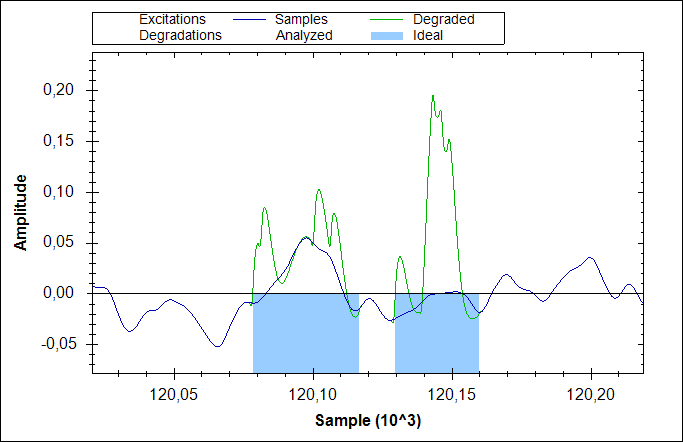
\includegraphics[width=0.75\textwidth]{images/znehodnotenia.png}
	\caption{Lokálne znehodnotenia}
	\label{obrazok:lokalne-znehodnotenia}
\end{figure}

\secwithtoc{Motivácia}
Pri pohľade na znehodnotené audio signály sa nám naskytla otázka, aká motivácia vedie k redukcii ich poškodenia? Dôvody môžu byť nasledujúce:
\begin{itemize}
	\item \textit{historické nahrávky} -- spomínaný záujem o reštaurovanie starších nahrávok, ktorý je diskutabilný z hľadiska odlišnosti názorov poslucháčov na prah rušivosti jednotlivých elementov. Niektorým poslucháčom starších nahrávok napríklad zvuk praskajúceho vinylu imponuje. Iným praskanie kazí zážitok z posluchu.
	\item \textit{neopakovateľné nahrávky} -- požadovaná kvalita autentických nahrávok, ktorých nahrávací proces je jedinečný a neopakovateľný. Ako príklad si veďme nahrávku z živého predstavenia, reportáže, koncertu alebo mimoriadnej udalosti.
	\item \textit{forenzná audio analýza} -- dôležitosť forenznej audio analýzy, ktorá je postavená na mechanizmoch reštaurovania audio signálu. Príkladom sú mechanizmy čistiace dôkazové materiály potrebné k napredovaniu súdnych procesov.
\end{itemize}

\secwithtoc{Cieľ práce}
V nasledujúcich kapitolách budeme uvažovať len digitálne signály a venovať sa budeme digitálnemu spracovaniu audio signálov. Konkrétne nás budú zaujímať mechanizmy detekcie a korekcie lokálnych znehodnotení digitálnych audio signálov s účelom reštaurovania poškodených nahrávok. Cieľom práce je vybrať, implementovať a subjektívne aj objektívne porovnať schopnosti a vlastnosti riešení danej problematiky.